\documentclass{article}
\usepackage{arxiv}
\usepackage[utf8]{inputenc}
\usepackage[T1]{fontenc}
\usepackage{hyperref}
\usepackage{url}
\usepackage{booktabs}
\usepackage{amsfonts}
\usepackage{amsmath}
\usepackage{graphicx}
\usepackage{float}
\usepackage[french]{babel}
\usepackage{subcaption}
\usepackage{enumitem}
\setlist{topsep=2pt,itemsep=1pt,leftmargin=*}

\usepackage{etoolbox}
\makeatletter
\patchcmd{\@maketitle}{\vskip 2em}{\vskip 0.5em}{}{}
\makeatother
\AtBeginDocument{
  \newgeometry{
    textheight=9.92in,
    textwidth=6.5in,
    top=0.6in,
    headheight=14pt,
    headsep=18pt,
    footskip=22pt
  }
}

\setlength{\abovecaptionskip}{4pt}
\setlength{\belowcaptionskip}{2pt}
\setlength{\textfloatsep}{6pt plus 2pt minus 2pt}
\setlength{\floatsep}{6pt plus 2pt minus 2pt}
\setlength{\intextsep}{6pt plus 2pt minus 2pt}
\setlength{\abovedisplayskip}{5pt}
\setlength{\belowdisplayskip}{5pt}
\title{Étude de l'impact des dynamiques non-déterministes sur l'évitement de situations dangereuses en apprentissage par renforcement}

\author{
  Abdelkarim Mouachiq \\
  Université Laval \\
  \texttt{abdelkarim.mouachiq.1@ulaval.ca} \\
  \And
  Saad ElGhissassi \\
  Université Laval \\
  \texttt{saad.elghissassi.1@ulaval.ca} \\
}

\begin{document}
\maketitle


\section{Cas d'étude}

L'environnement Frozen Lake (v1) de la librairie Gymnasium~\cite{towers2024gymnasium} modélise un lac gelé que l'agent doit traverser pour atteindre un objectif tout en évitant des trous. Chaque cellule de la grille est de l'un des types suivants~: départ (\texttt{S}), surface gelée (\texttt{F}), trou (\texttt{H}) ou objectif (\texttt{G}). L'agent dispose de quatre actions~: gauche, bas, droite et haut. En mode glissant, chaque action a une probabilité de $\frac{1}{3}$ de déplacer l'agent dans la direction voulue et $\frac{1}{3}$ pour chacune des deux directions perpendiculaires. L'agent reçoit une récompense de $+1$ s'il atteint l'objectif et $0$ dans tous les autres cas (chute dans un trou ou dépassement de la limite de pas). Un épisode se termine lorsque l'agent atteint l'objectif, tombe dans un trou, ou dépasse la limite de pas (100 pour le cas~1, 200 pour les cas~2 et~3). Il n'y a donc aucune pénalité explicite pour les chutes~: la seule incitation est la récompense positive à l'objectif.

\subsection{Ajustement de la difficulté}

Trois paramètres permettent d'ajuster la difficulté~:
\begin{itemize}
    \item \textbf{Stochasticité~:} le paramètre de glissement contrôle si les transitions sont déterministes ou stochastiques, rendant l'évitement des trous plus imprévisible.
    \item \textbf{Nombre de trous~:} une proportion élevée de trous réduit les chemins sûrs disponibles.
    \item \textbf{Positionnement des trous~:} des trous placés près du chemin optimal forcent l'agent dans des corridors étroits, augmentant le risque de chute lors de l'apprentissage.
\end{itemize}

\subsection{Description et motivation des cas d'étude}

Nous proposons trois cas de difficulté croissante, tous en mode stochastique~:

\textbf{Cas~1~: Simple (4$\times$4, 1 trou, 6.25\% de danger).} Grille de 16 cases avec un unique trou en position (1,1). Ce cas isole l'effet de la stochasticité~: la difficulté provient uniquement du glissement, pas de la densité des obstacles.

\textbf{Cas~2~: Modéré (8$\times$8, 10 trous, 15.6\% de danger).} Les trous sont concentrés dans les lignes 3 à 8, créant une zone haute dégagée et une zone basse avec des corridors étroits. Ce design teste le compromis exploration/sécurité.

\textbf{Cas~3~: Difficile (8$\times$8, 17 trous, 26.6\% de danger).} Les trous sont répartis sur l'ensemble de la grille. Il existe des chemins viables de \texttt{S} vers \texttt{G} (la grille est solvable en mode déterministe), mais chaque chemin passe par des cellules adjacentes à un ou plusieurs trous. Certains chemins sont plus sécuritaires que d'autres (passant par moins de cellules à risque), ce qui permet d'évaluer si une stratégie est capable d'identifier et privilégier ces chemins malgré le glissement stochastique. La figure~\ref{fig:study_cases} illustre les trois configurations.

\begin{figure}[H]
    \centering
    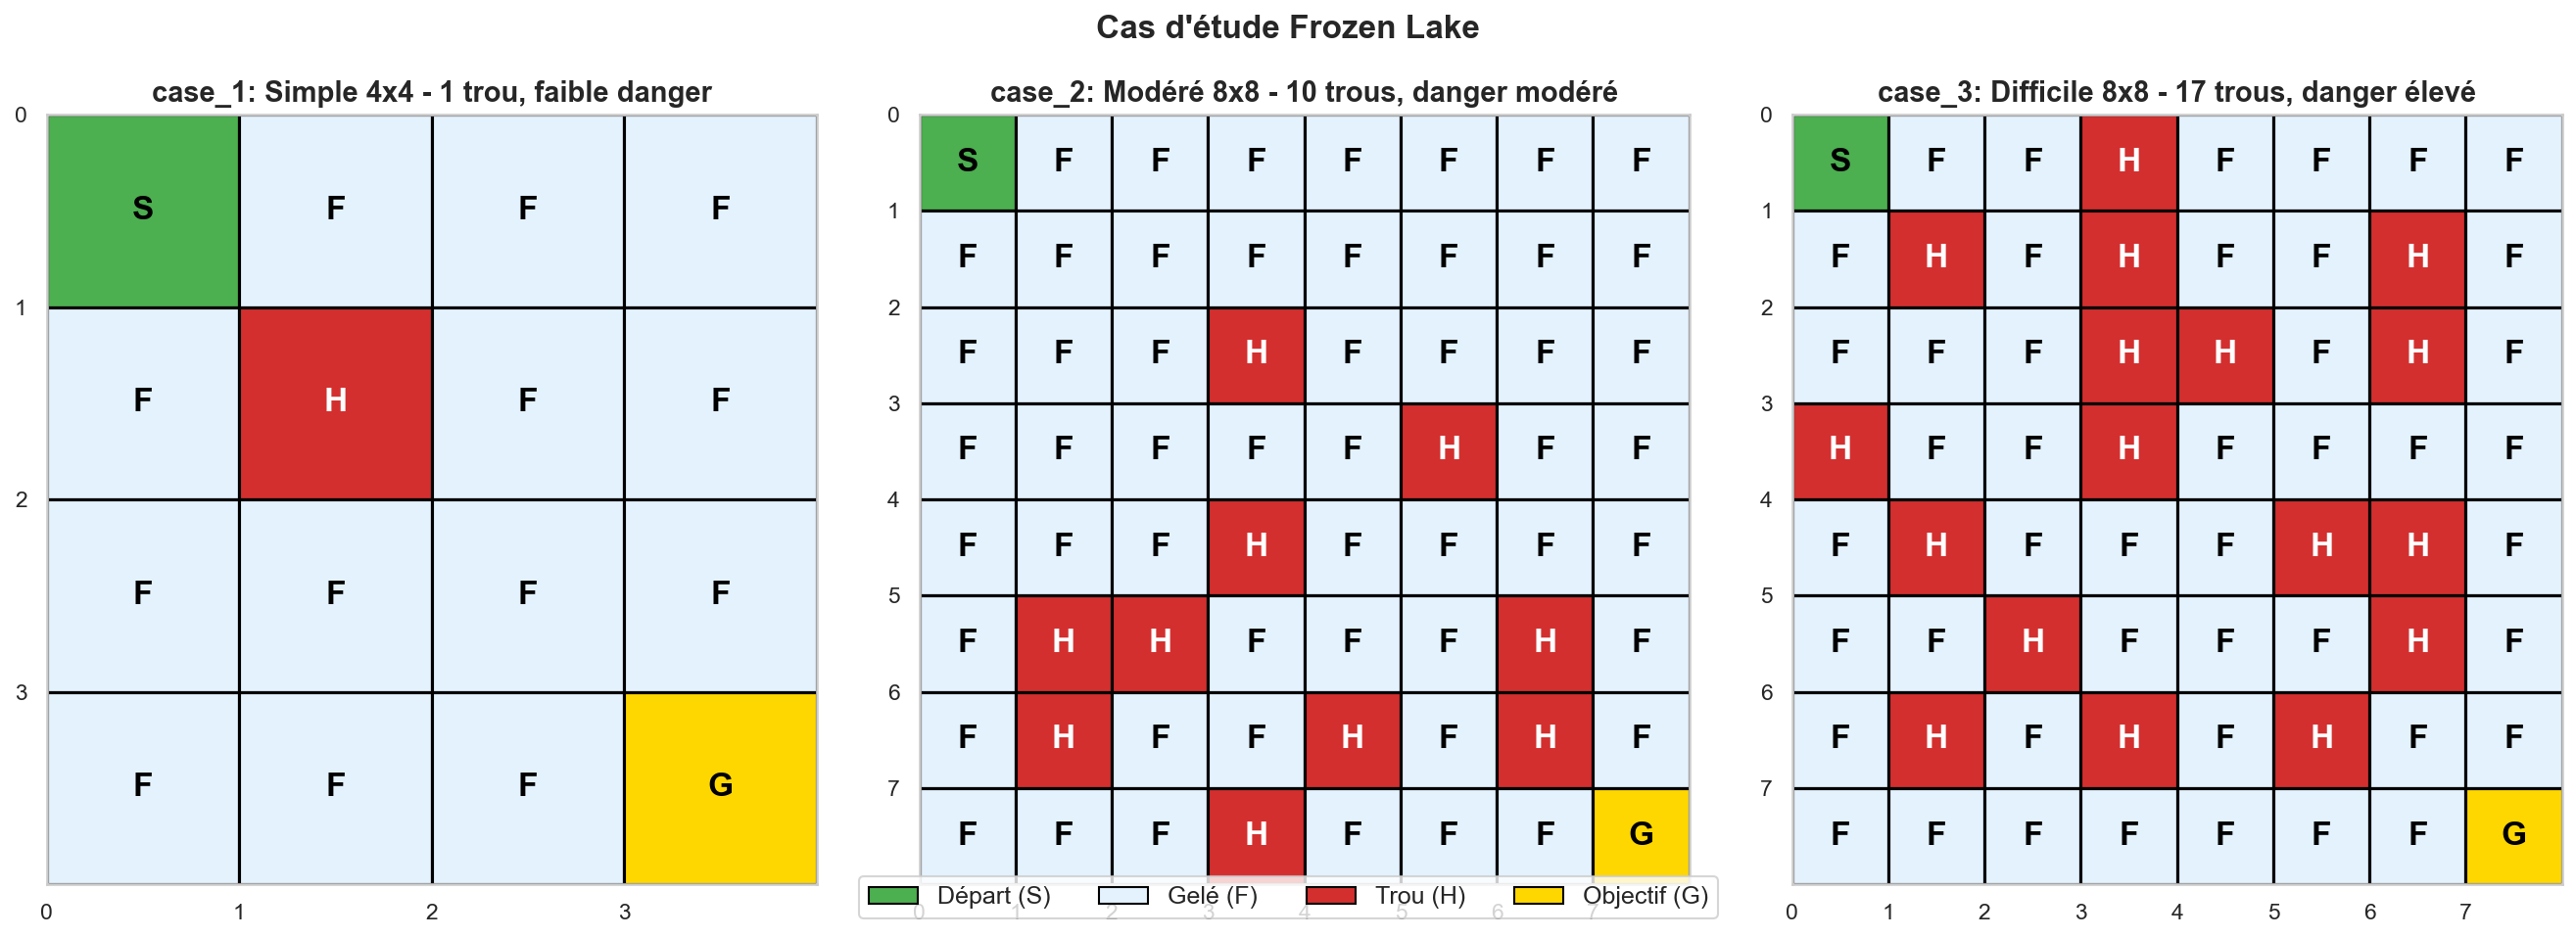
\includegraphics[width=0.8\textwidth]{figures/study_cases.png}
    \caption{Configurations des trois cas d'étude. Vert~: départ, bleu~: gelé, rouge~: trou, jaune~: objectif.}
    \label{fig:study_cases}
\end{figure}


\section{Stratégies considérées}

\subsection{Stratégies de référence}

Nous comparons deux stratégies qui ne sont pas conçues pour gérer les situations dangereuses.

\subsubsection{DQN (Deep Q-Network)}

DQN~\cite{mnih2015human} est un algorithme \textit{off-policy} qui approxime la fonction de valeur d'action $Q(s,a)$ via un réseau de neurones. Il apprend la politique optimale (gloutonne) tout en suivant une politique d'exploration différente ($\varepsilon$-gloutonne), grâce à un tampon de rejeu d'expérience qui stocke les transitions passées. Un réseau cible $\theta^-$, mis à jour périodiquement, stabilise l'apprentissage. La perte minimisée est~:
\begin{equation}
\mathcal{L}(\theta) = \mathbb{E}_{(s,a,r,s') \sim \mathcal{D}} \left[ \left( r + \gamma \max_{a'} Q(s', a'; \theta^-) - Q(s,a;\theta) \right)^2 \right]
\end{equation}

\textbf{Motivation~:} DQN est le standard en RL profond basé sur la valeur. Son caractère \textit{off-policy} lui permet de réutiliser les expériences passées, ce qui devrait le rendre efficace en termes d'échantillons. Cependant, l'utilisation d'un réseau de neurones pour approximer $Q$ est surdimensionnée pour Frozen Lake, où l'espace d'états est petit (16 ou 64 états discrets). Le réseau reçoit un scalaire en entrée et peine à distinguer des états sans structure spatiale, contrairement à une approche tabulaire qui apprend chaque état indépendamment. Nous incluons néanmoins DQN pour illustrer cette limitation et parce qu'il représente l'approche standard en RL profond.

\subsubsection{PPO (Proximal Policy Optimization)}

PPO~\cite{schulman2017proximal} est un algorithme \textit{on-policy} qui optimise directement la politique $\pi_\theta(a|s)$. Contrairement à DQN, PPO utilise uniquement les données collectées par la politique courante, puis les jette après chaque mise à jour. L'objectif avec troncature est~:
\begin{equation}
\mathcal{L}^{\text{CLIP}}(\theta) = \hat{\mathbb{E}}_t \left[ \min\left( r_t(\theta) \hat{A}_t, \; \text{clip}(r_t(\theta), 1{-}\epsilon, 1{+}\epsilon) \hat{A}_t \right) \right]
\end{equation}
où $r_t(\theta) = \pi_\theta(a_t|s_t) / \pi_{\theta_{\text{old}}}(a_t|s_t)$ et $\hat{A}_t$ est l'estimateur d'avantage généralisé (EAG).

\textbf{Motivation~:} PPO représente la famille des méthodes de gradient de politique, complémentaire à DQN (basé sur la valeur). Son caractère \textit{on-policy} le rend plus stable mais moins efficace en échantillons. Comme DQN, il ne dispose d'aucun mécanisme pour éviter les états dangereux durant l'exploration.

\subsection{Approches de la littérature en RL sécuritaire}

Nous avons identifié trois articles proposant des méthodes adaptées à l'évitement de situations dangereuses~:

\paragraph{1. Optimisation de politique sous contraintes (CPO)~\cite{achiam2017constrained}.} CPO formule le RL sécuritaire comme un processus de décision markovien contraint (CMDP) où l'agent maximise la récompense sous une contrainte de coût cumulative. L'algorithme effectue des mises à jour de politique dans une région de confiance définie par une approximation de second ordre, garantissant théoriquement que chaque mise à jour améliore la performance tout en respectant les contraintes de sécurité. CPO cible les politiques paramétriques et a été validé sur des tâches de locomotion continue.

\paragraph{2. Couche de sécurité pour l'exploration~\cite{dalal2018safe}.} Cette approche intercale une couche de correction entre la politique et l'environnement. À chaque pas, l'action proposée par la politique est projetée sur l'ensemble des actions satisfaisant les contraintes de sécurité via la résolution d'un programme linéaire. Un modèle linéaire de la dynamique, appris en ligne, prédit si une action mènera à une violation de contrainte. La projection garantit que l'action exécutée est la plus proche (au sens $L_2$) de l'action originale tout en étant sûre. Cette méthode requiert un espace d'actions continu pour la projection et n'est donc pas applicable aux environnements à actions discrètes comme Frozen Lake.

\paragraph{3. RL sécuritaire dans les CMDP~\cite{wachi2020safe}.} Wachi et Sui proposent un algorithme pour les CMDP qui sépare explicitement l'estimation de la récompense et du coût en deux fonctions de valeur distinctes. Contrairement à CPO qui intègre la contrainte dans la mise à jour de politique, cette approche modélise l'incertitude sur la fonction de coût via un processus gaussien, ce qui permet de construire un ensemble d'actions sûres avec garantie probabiliste. L'agent explore de manière conservatrice en évitant les régions où l'incertitude sur le coût est élevée, optimisant la récompense uniquement parmi les actions jugées sûres. Cette séparation récompense/coût est directement applicable aux environnements discrets.

\subsection{Stratégie sélectionnée~: Safe Q-Learning}

Nous implémentons l'approche de Q-Learning contraint décrite par García et Fernández~\cite{garcia2015comprehensive} (section~4.2, \textit{constrained criterion}). Cette section décrit un agent tabulaire qui maintient deux fonctions de valeur (récompense et coût) et sélectionne ses actions en filtrant celles dont le coût estimé dépasse un seuil — le cadre exact des CMDP tabulaires. Ce principe est partagé par Wachi et Sui~\cite{wachi2020safe} qui l'étendent aux espaces continus via des processus gaussiens. Notre contribution spécifique est l'initialisation de la table de coût $Q_c$ avec le modèle de transitions connu de Frozen Lake (non décrite dans~\cite{garcia2015comprehensive}), ce qui permet d'éviter les dangers dès le début de l'apprentissage. Les trois composantes sont~:

\textbf{1. Double table de valeurs.} L'agent maintient $Q_r(s,a)$ pour la récompense et $Q_c(s,a)$ pour le coût (probabilité de chute). Les mises à jour suivent~:
\begin{align}
Q_r(s,a) &\leftarrow Q_r(s,a) + \alpha_r \left[ r + \gamma_r \max_{a'} Q_r(s', a') - Q_r(s,a) \right] \\
Q_c(s,a) &\leftarrow Q_c(s,a) + \alpha_c \left[ c + \gamma_c \max_{a'} Q_c(s', a') - Q_c(s,a) \right]
\end{align}
où $c = 1$ si l'agent tombe dans un trou, $0$ sinon. Le facteur $\gamma_c = 0.5$ (vs $\gamma_r = 0.99$) favorise la sensibilité au danger immédiat.

\textbf{2. Exploration contrainte.} L'agent filtre les actions dont $Q_c(s,a) > \tau$ et applique une politique $\varepsilon$-gloutonne sur $Q_r$ parmi les actions sûres restantes~: $a = \arg\max_{a \in \mathcal{A}_{\text{sûr}}(s)} Q_r(s,a)$ où $\mathcal{A}_{\text{sûr}}(s) = \{a : Q_c(s,a) < \tau\}$.

\textbf{3. Initialisation du modèle de coût.} En exploitant le modèle de transitions connu, $Q_c$ est initialisé avec les probabilités de transition vers les trous, permettant d'éviter les dangers dès le début.

\textbf{Justification du choix~:} le Q-Learning contraint décrit par~\cite{garcia2015comprehensive} est directement applicable aux environnements discrets tabulaires. CPO~\cite{achiam2017constrained} requiert une politique paramétrique et la couche de sécurité~\cite{dalal2018safe} nécessite un espace d'actions continu — aucun des deux n'est applicable à Frozen Lake sans modification majeure.


\section{Méthodologie expérimentale}

\subsection{Hyper-paramètres}

DQN et PPO sont implémentés via Stable-Baselines3~\cite{raffin2021stable}; le Q-Learning et le Safe Q-Learning sont implémentés manuellement. Les hyper-paramètres (tableaux~\ref{tab:dqn_params} et~\ref{tab:safe_ql_params}) ont été déterminés par recherche sur grille sur le cas~1 puis ajustés.

\begin{table}[H]
\centering
\caption{Hyper-paramètres de DQN et PPO.}
\label{tab:dqn_params}
\small
\begin{tabular}{lcccccc}
\toprule
 & \multicolumn{3}{c}{\textbf{DQN}} & \multicolumn{3}{c}{\textbf{PPO}} \\
\cmidrule(lr){2-4} \cmidrule(lr){5-7}
Paramètre & C1 & C2 & C3 & C1 & C2 & C3 \\
\midrule
Taux d'apprentissage & $10^{-3}$ & $5{\times}10^{-4}$ & $5{\times}10^{-4}$ & $3{\times}10^{-4}$ & $3{\times}10^{-4}$ & $3{\times}10^{-4}$ \\
$\gamma$ & 0.99 & 0.99 & 0.99 & 0.99 & 0.99 & 0.99 \\
Taille du lot & 64 & 128 & 128 & 64 & 128 & 128 \\
$\varepsilon$ final / Coeff. entropie & 0.05 & 0.05 & 0.05 & 0.01 & 0.01 & 0.02 \\
Pas de temps totaux & 50k & 100k & 150k & 50k & 100k & 150k \\
\bottomrule
\end{tabular}
\end{table}

\begin{table}[H]
\centering
\caption{Hyper-paramètres du Q-Learning standard et Safe Q-Learning.}
\label{tab:safe_ql_params}
\small
\begin{tabular}{lcccccc}
\toprule
 & \multicolumn{3}{c}{\textbf{Q-Learning}} & \multicolumn{3}{c}{\textbf{Safe Q-Learning}} \\
\cmidrule(lr){2-4} \cmidrule(lr){5-7}
Paramètre & C1 & C2 & C3 & C1 & C2 & C3 \\
\midrule
$\alpha$ (récompense) & 0.1 & 0.1 & 0.1 & 0.1 & 0.1 & 0.1 \\
$\alpha_c$ (coût) & -- & -- & -- & 0.2 & 0.15 & 0.15 \\
$\gamma_r$ / $\gamma_c$ & 0.99 & 0.99 & 0.99 & 0.99 / 0.5 & 0.99 / 0.5 & 0.99 / 0.5 \\
Seuil $\tau$ & -- & -- & -- & 0.3 & 0.35 & 0.4 \\
Épisodes & 20k & 50k & 80k & 20k & 50k & 80k \\
\bottomrule
\end{tabular}
\end{table}

\subsection{Indicateurs de performance}

\begin{itemize}
    \item \textbf{Taux de succès~:} proportion d'épisodes d'évaluation où l'agent atteint l'objectif.
    \item \textbf{Taux de chutes (évaluation)~:} proportion d'épisodes d'évaluation terminés par une chute.
    \item \textbf{Taux de chutes cumulatif (entraînement)~:} ratio chutes/épisodes \textit{durant} l'apprentissage, quantifiant le coût en situations dangereuses.
    \item \textbf{Récompense moyenne~:} récompense moyenne sur les épisodes d'évaluation.
\end{itemize}

\subsection{Paramètres expérimentaux}

Chaque expérience est répétée avec 5 graines aléatoires (42, 123, 456, 789, 1024). L'évaluation est effectuée périodiquement sur 20 à 50 épisodes en mode déterministe. Le code source est structuré en modules documentés (\texttt{environment.py}, \texttt{train\_baselines.py}, \texttt{train\_safe\_rl.py}, \texttt{run\_all\_experiments.py}) avec un fichier \texttt{requirements.txt}~: \url{https://github.com/Karimartcode/Frozen_Lake_RL}.


\section{Résultats}

\subsection{Performance finale}

Le tableau~\ref{tab:all_results} présente les performances finales de toutes les stratégies.

\begin{table}[H]
\centering
\caption{Comparaison des performances de toutes les stratégies (moyenne $\pm$ écart-type, 5 graines).}
\label{tab:all_results}
\resizebox{\textwidth}{!}{
\begin{tabular}{llcccc}
\toprule
Stratégie & Cas & Taux de succès & Taux de chutes (éval.) & Taux de chutes (entr.) & Récomp. moy. \\
\midrule
DQN & Cas 1 & $100.0 \pm 0.0\%$ & $0.0 \pm 0.0\%$ & $52.6 \pm 3.9\%$ & $1.000 \pm 0.000$ \\
DQN & Cas 2 & $37.0 \pm 19.6\%$ & $13.0 \pm 10.8\%$ & $59.8 \pm 1.2\%$ & $0.370 \pm 0.196$ \\
DQN & Cas 3 & $0.0 \pm 0.0\%$ & $100.0 \pm 0.0\%$ & $99.9 \pm 0.0\%$ & $0.000 \pm 0.000$ \\
\midrule
PPO & Cas 1 & $100.0 \pm 0.0\%$ & $0.0 \pm 0.0\%$ & $24.8 \pm 4.8\%$ & $1.000 \pm 0.000$ \\
PPO & Cas 2 & $29.0 \pm 28.5\%$ & $13.0 \pm 16.6\%$ & $60.8 \pm 15.8\%$ & $0.290 \pm 0.285$ \\
PPO & Cas 3 & $0.0 \pm 0.0\%$ & $100.0 \pm 0.0\%$ & $100.0 \pm 0.0\%$ & $0.000 \pm 0.000$ \\
\midrule
Q-Learning & Cas 1 & $100.0 \pm 0.0\%$ & $0.0 \pm 0.0\%$ & $57.7 \pm 0.3\%$ & $1.000 \pm 0.000$ \\
Q-Learning & Cas 2 & $62.0 \pm 5.2\%$ & $9.6 \pm 7.3\%$ & $60.6 \pm 0.2\%$ & $0.620 \pm 0.052$ \\
Q-Learning & Cas 3 & $0.0 \pm 0.0\%$ & $100.0 \pm 0.0\%$ & $100.0 \pm 0.0\%$ & $0.000 \pm 0.000$ \\
\midrule
Safe Q-Learning & Cas 1 & $100.0 \pm 0.0\%$ & $0.0 \pm 0.0\%$ & $0.0 \pm 0.0\%$ & $1.000 \pm 0.000$ \\
Safe Q-Learning & Cas 2 & $52.0 \pm 4.6\%$ & $15.2 \pm 4.5\%$ & $19.1 \pm 0.1\%$ & $0.520 \pm 0.046$ \\
Safe Q-Learning & Cas 3 & $0.8 \pm 1.0\%$ & $95.6 \pm 1.5\%$ & $96.8 \pm 0.1\%$ & $0.008 \pm 0.010$ \\
\bottomrule
\end{tabular}}
\end{table}


Les récompenses moyennes (tableau~\ref{tab:all_results}) reflètent directement les taux de succès puisque la seule récompense positive est +1 à l'objectif. Sur le cas~1, toutes les stratégies atteignent 100\% de succès. La différence majeure réside dans le coût d'apprentissage~: DQN et Q-Learning enregistrent respectivement 52.6\% et 57.7\% de chutes durant l'entraînement, tandis que le Safe Q-Learning élimine totalement les chutes (0\%). Sur le cas~2, le Q-Learning tabulaire domine (62\% de succès) devant le Safe Q-Learning (52\%), DQN (37\%) et PPO (29\%). Le Safe Q-Learning réduit le taux de chutes d'entraînement de $\sim$60\% à 19\%. Sur le cas~3, aucune stratégie ne résout l'environnement~: les taux de succès sont à 0\% (sauf Safe Q-Learning à 0.8\%).

\subsection{Courbes d'apprentissage}

La figure~\ref{fig:all_success} montre l'évolution du taux de succès. Sur le cas~1, DQN présente des oscillations marquées avant de se stabiliser vers 50\,000 pas, contrairement aux méthodes tabulaires qui convergent plus tôt. Sur le cas~2, la variance inter-graines est élevée pour toutes les stratégies, avec le Q-Learning tabulaire atteignant les meilleurs résultats. Le cas~3 confirme l'absence de convergence.

\begin{figure}[H]
    \centering
    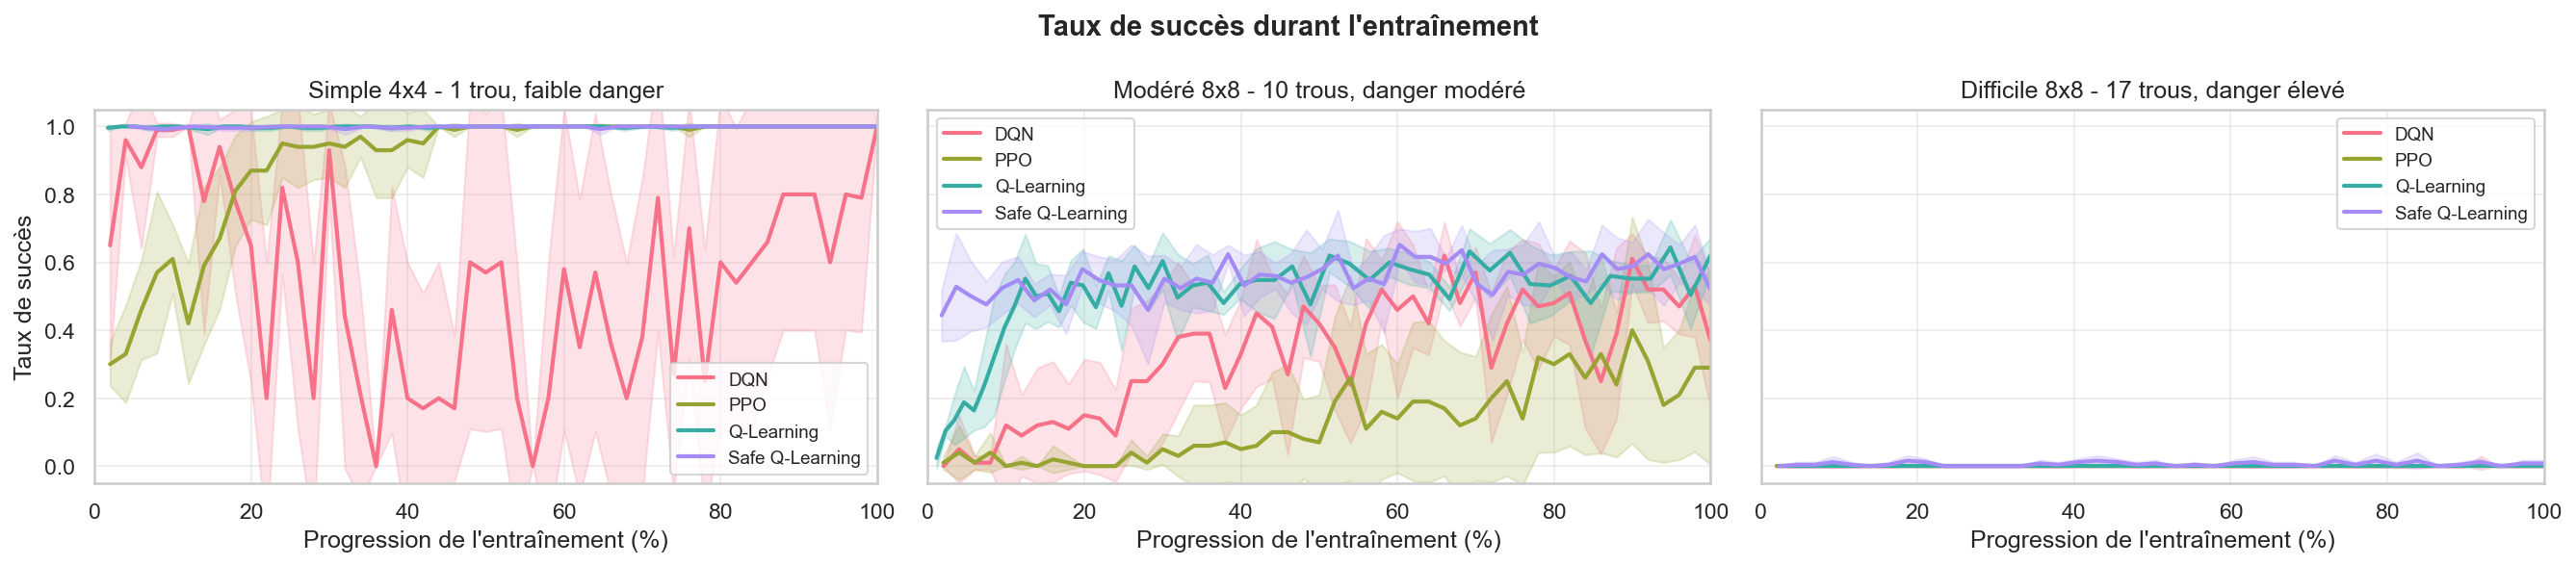
\includegraphics[width=0.7\textwidth]{figures/all_success_rate.png}
    \caption{Taux de succès durant l'entraînement (moyenne $\pm$ écart-type, 5 graines). L'axe X est normalisé en pourcentage de la durée totale d'entraînement pour permettre la comparaison entre les cas.}
    \label{fig:all_success}
\end{figure}

La figure~\ref{fig:all_hole_eval} montre le taux de chutes en évaluation. Sur le cas~1, toutes les stratégies éliminent les chutes en fin d'entraînement. Sur le cas~2, DQN et PPO conservent 13\% de chutes tandis que le Q-Learning tabulaire descend à 9.6\%. Sur le cas~3, toutes les stratégies atteignent $\sim$100\% de chutes sauf le Safe Q-Learning (95.6\%).

\begin{figure}[H]
    \centering
    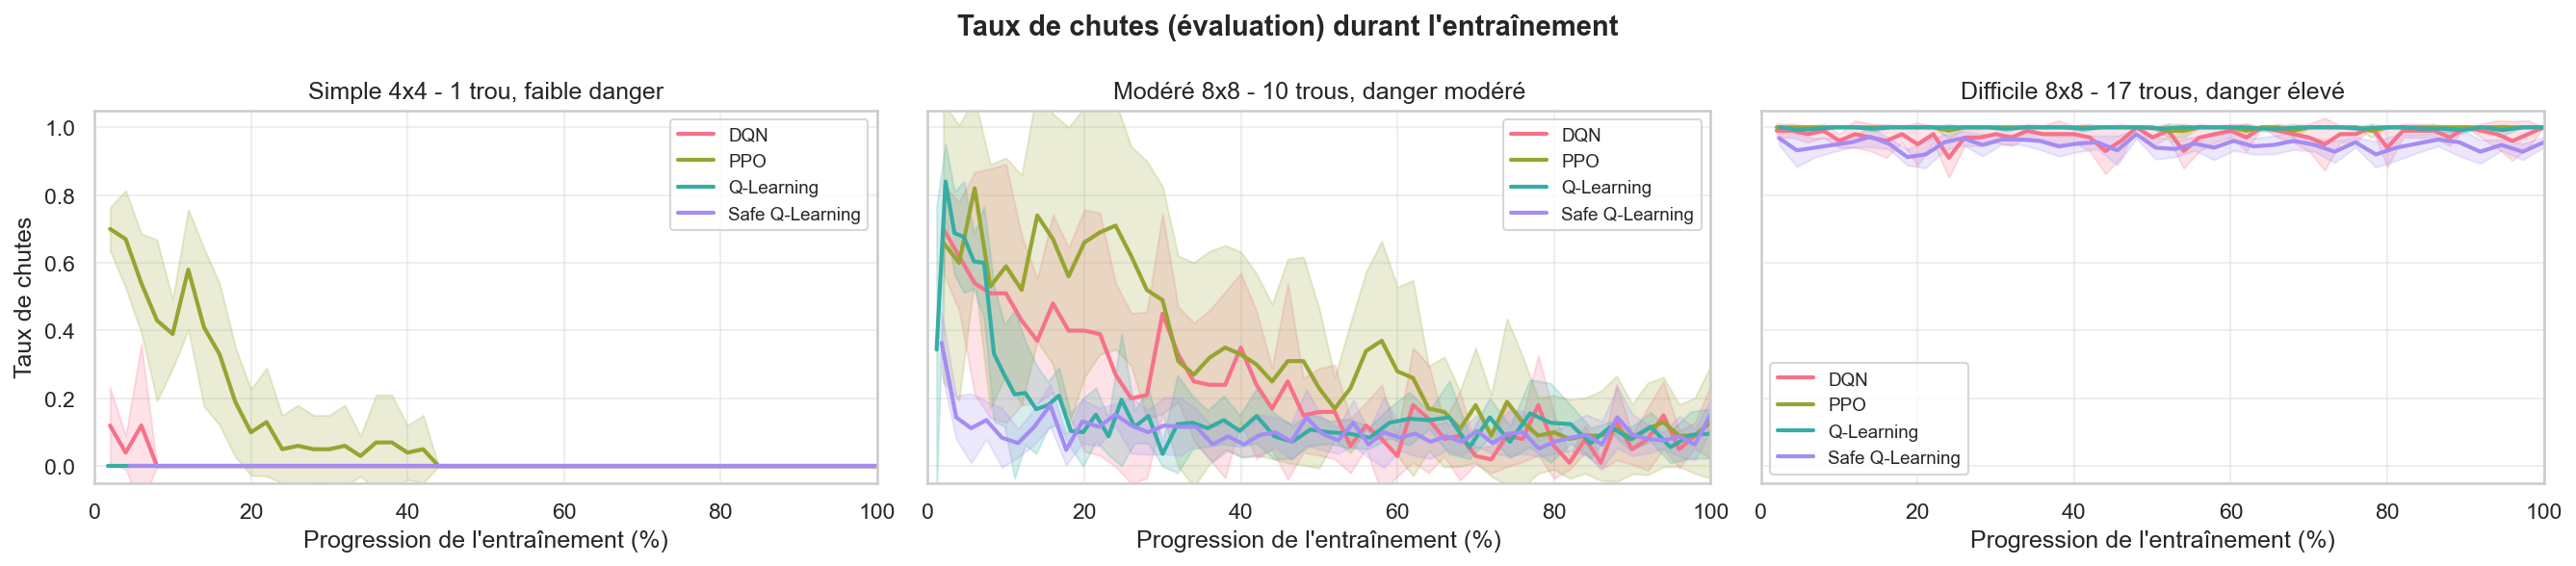
\includegraphics[width=0.7\textwidth]{figures/all_hole_rate.png}
    \caption{Taux de chutes en évaluation durant l'entraînement.}
    \label{fig:all_hole_eval}
\end{figure}

La figure~\ref{fig:all_train_holes} montre le taux de chutes cumulatif (indicateur clé de sécurité). Le Safe Q-Learning maintient 0\% de chutes sur le cas~1 et 19\% sur le cas~2, contre $\sim$60\% pour les autres. La récompense moyenne (non illustrée, cf. tableau~\ref{tab:all_results}) reflète directement les taux de succès.

\begin{figure}[H]
    \centering
    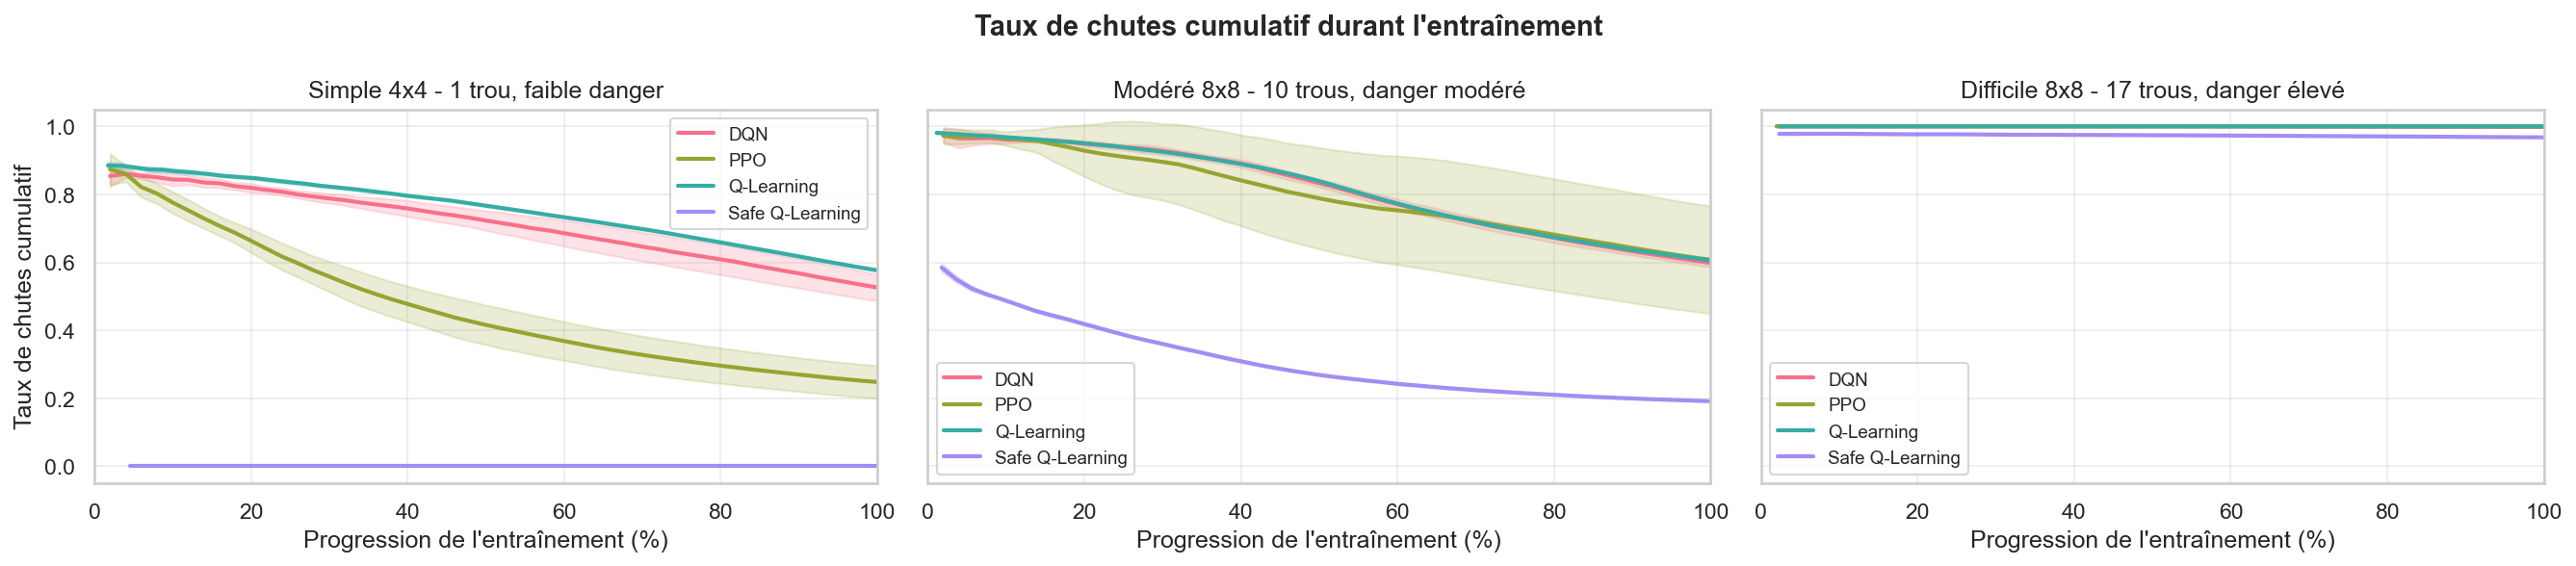
\includegraphics[width=0.7\textwidth]{figures/all_train_hole_rate.png}
    \caption{Taux de chutes cumulatif durant l'entraînement.}
    \label{fig:all_train_holes}
\end{figure}

\subsection{Politiques apprises}

Sur le cas~1 (figure~\ref{fig:all_policy_1}), le Safe Q-Learning s'éloigne davantage du trou, reflétant son exploration conservatrice. Sur le cas~2 (figure~\ref{fig:all_policy_2}), seules les méthodes tabulaires trouvent des chemins cohérents à travers les corridors. Sur le cas~3 (non illustré car aucune stratégie n'atteint l'objectif), les politiques sont aléatoires. Les visualisations haute résolution des trois cas sont disponibles dans le dépôt GitHub.

\begin{figure}[H]
    \centering
    \begin{subfigure}[t]{0.45\textwidth}
        \centering
        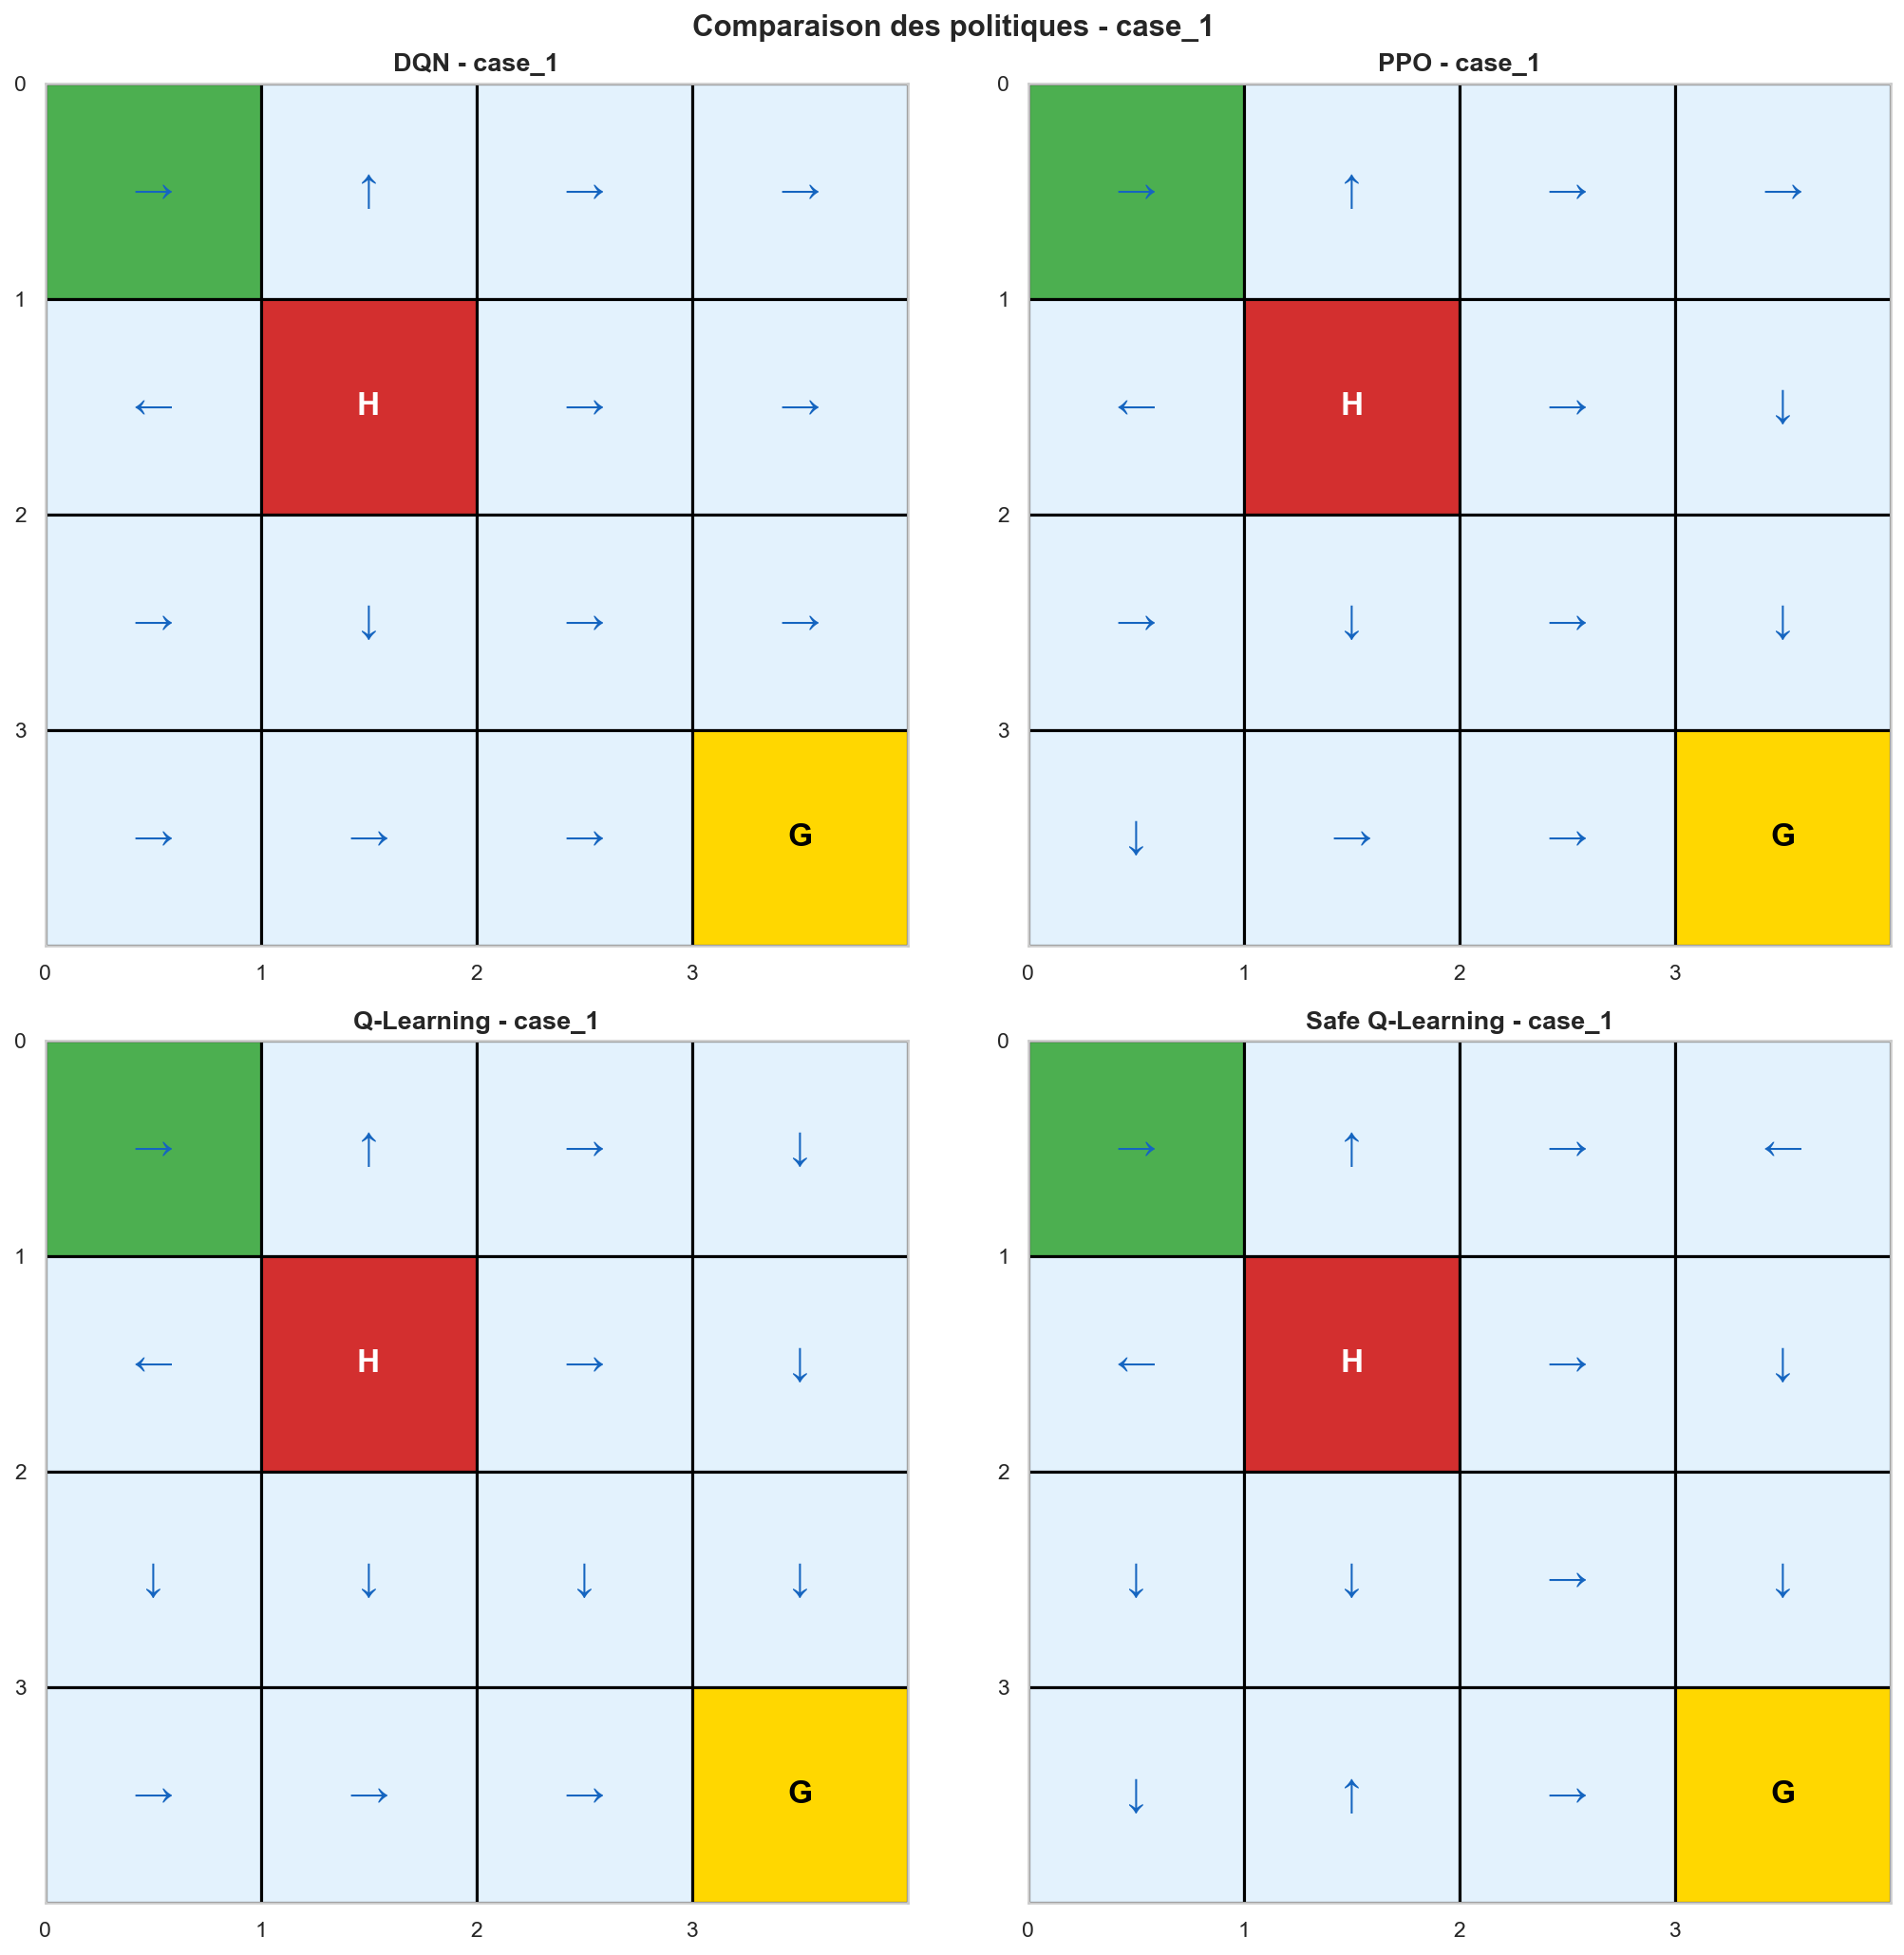
\includegraphics[width=\textwidth]{figures/all_policy_case_1.png}
        \caption{Cas~1}
        \label{fig:all_policy_1}
    \end{subfigure}
    \hfill
    \begin{subfigure}[t]{0.45\textwidth}
        \centering
        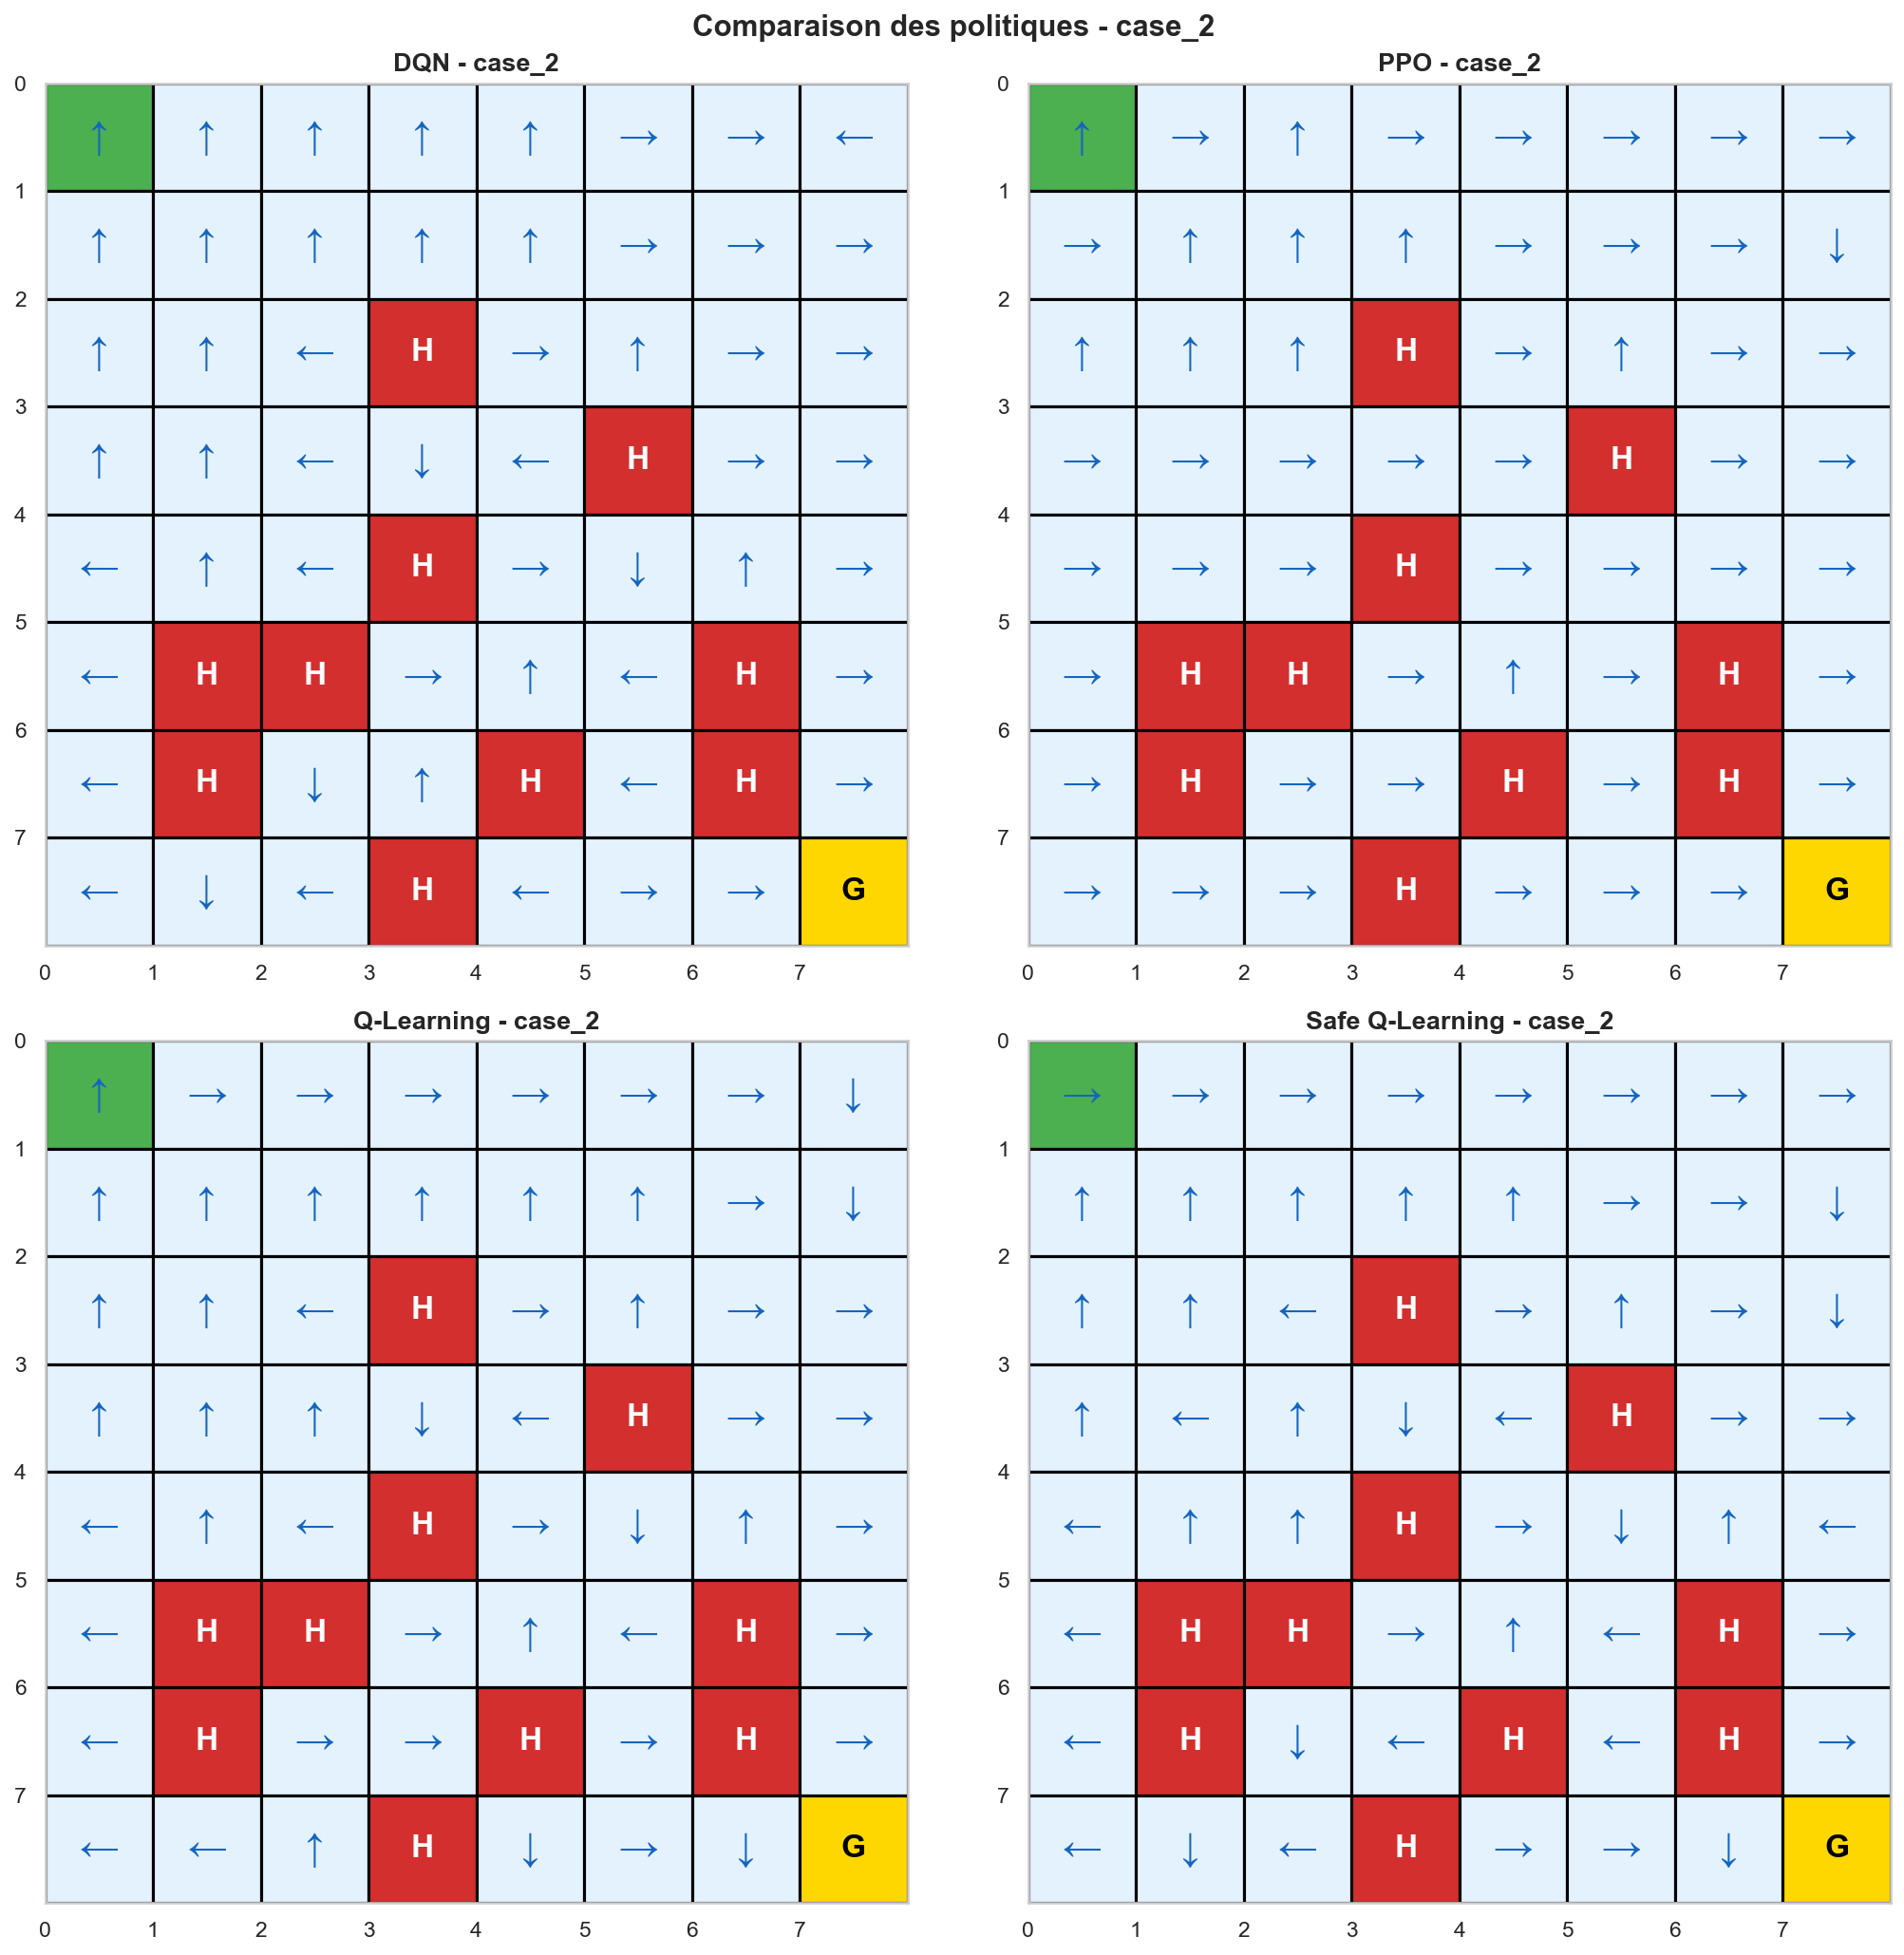
\includegraphics[width=\textwidth]{figures/all_policy_case_2.png}
        \caption{Cas~2}
        \label{fig:all_policy_2}
    \end{subfigure}
    \caption{Politiques apprises par les 4 stratégies (disposition 2$\times$2 pour lisibilité).}
    \label{fig:all_policies}
\end{figure}


\section{Discussion}

\subsection{Liens avec la littérature}

Nos résultats confirment le compromis fondamental entre performance et sécurité identifié par García et Fernández~\cite{garcia2015comprehensive}~: une exploration conservatrice réduit les chutes mais peut empêcher la découverte de politiques optimales. Sur le cas~2, le Safe Q-Learning réduit le taux de chutes d'entraînement de 60\% à 19\%, mais son taux de succès final (52\%) reste inférieur à celui du Q-Learning standard (62\%). Ce compromis est cohérent avec les résultats de Wachi et Sui~\cite{wachi2020safe}, qui observent que les contraintes de sécurité limitent l'exploration des régions à haute récompense.

L'efficacité de l'initialisation de $Q_c$ confirme l'observation d'Achiam et al.~\cite{achiam2017constrained} selon laquelle l'exploitation de connaissances \textit{a priori} sur les contraintes accélère considérablement la convergence vers une politique sûre. La supériorité des méthodes tabulaires sur les méthodes profondes s'explique par la nature de l'espace d'états~: un entier discret encodant la position. Les réseaux de neurones de DQN et PPO reçoivent un scalaire en entrée et peinent à distinguer des états qui ne partagent aucune structure. Une approche tabulaire apprend chaque état indépendamment, sans risque d'interférence entre les mises à jour. Ce constat illustre l'importance du choix de la représentation d'état~\cite{mnih2015human}.

\subsection{Explication des résultats}

\textbf{Oscillations de DQN sur le cas~1~:} le réseau approxime $Q(s,a)$ pour les 16 états simultanément. Une mise à jour des poids pour un état peut dégrader les estimations des autres (interférence catastrophique), expliquant les oscillations malgré la simplicité de l'environnement.

\textbf{Supériorité du Q-Learning tabulaire sur le cas~2~:} avec 64 états, la table Q ($64 \times 4 = 256$ entrées) apprend chaque état indépendamment, sans interférence. Son caractère \textit{off-policy} lui permet de réutiliser les transitions, contrairement à PPO qui jette ses données après chaque mise à jour.

\textbf{Cas~3 insoluble~:} tout chemin traverse des cellules adjacentes à des trous. La probabilité de compléter un chemin de longueur $L$ sans chute est $(1 - p_{\text{chute}})^L$. Pour $L = 14$ et $p_{\text{chute}} \approx 0.15$~: $(0.85)^{14} \approx 10\%$. Les baselines ne suffisent pas, et même le Safe Q-Learning n'atteint que 0.8\%.

\textbf{Safe Q-Learning sans chutes sur le cas~1~:} l'initialisation de $Q_c$ avec le modèle de transitions connu permet d'éviter le trou dès le début. Avec $\tau = 0.3$, l'agent filtre systématiquement les actions dangereuses.

\subsection{Réflexion sur les approches}

En termes de complexité algorithmique, les méthodes tabulaires requièrent $O(|\mathcal{S}||\mathcal{A}|)$ opérations par mise à jour et s'entraînent en quelques secondes, contre plusieurs minutes pour DQN ($O(d^2)$ par passe réseau) et PPO. Pour des espaces d'états continus ou de haute dimension, CPO~\cite{achiam2017constrained} ou la couche de sécurité~\cite{dalal2018safe} seraient nécessaires malgré leur coût computationnel supérieur.

Le seuil $\tau$ contrôle directement le compromis sécurité/performance. Avec $\tau = 0.35$ sur le cas~2, le Safe Q-Learning atteint 52\% de succès. Un $\tau$ plus bas ($0.2$) filtrerait trop d'actions dans les corridors où le glissement rend toutes les actions partiellement dangereuses, abaissant le taux de succès. Un $\tau$ plus élevé ($0.5$) serait plus permissif mais offrirait moins de protection. Un mécanisme d'ajustement adaptatif de $\tau$ (décroissant à mesure que $Q_c$ se stabilise) pourrait améliorer ce compromis sans calibration manuelle.

L'initialisation de $Q_c$ via le modèle de transitions est un avantage spécifique aux environnements à modèle connu. Dans un environnement réel où ce modèle n'est pas disponible, $Q_c$ devrait être appris de zéro, réduisant l'avantage de sécurité initial. L'utilisation d'un modèle approximatif appris en ligne pourrait servir de compromis.

\subsection{Message au client}

Les stratégies classiques de RL (DQN, PPO) enregistrent plus de 50\% de chutes durant l'apprentissage même lorsque la politique finale est performante. Nos recommandations~:
\begin{enumerate}
    \item \textbf{Intégrer un modèle de coût~:} une double fonction de valeur permet de filtrer les actions dangereuses durant l'exploration, réduisant les chutes de 60\% à 19\%.
    \item \textbf{Exploiter la connaissance disponible~:} initialiser les estimations de danger avec le modèle de transitions élimine les incidents en début d'apprentissage.
    \item \textbf{Adapter la représentation~:} les approches tabulaires surpassent les réseaux de neurones dans les environnements discrets de taille modeste.
    \item \textbf{Évaluer la faisabilité~:} dans les environnements très denses en dangers, envisager un pré-entraînement en simulation, un apprentissage par démonstration, ou des méthodes de blindage.
\end{enumerate}

\newpage
\bibliographystyle{plain}
\bibliography{references}

\end{document}
